\documentclass[12pt,fleqn]{article}\usepackage{../common}
\begin{document}

Ders 2

Gercek dunyada cogu ODE sayisal (numerical) yontemlerle
cozulur. Bilgisayarinizda bir ODE'yi grafiklettirdiginiz zaman da aslinda arka
planda bilgisayar o denklemi sayisal olarak cozmekte ve sonucu
grafiklettirmektedir. Bir baslangic degerli (initial value) probleminin formunu
yazalim: 

\[ y' = f(x,y) \]

\[ y_1(x_o) = y_o \]

Problemde ilk satir ODE, ikinci satir bu ODE'nin baslangic degeri, $x_0$ ve $y_0$
sabit degerler. 

Numerik olarak (mesela Euler yontemiyle) bu denklemi cozmek ne demektir? Alttaki
cizime bakalim, $y_0$'dan degerinden basliyoruz, bu noktada $x_0,y_0$
noktasindaki egimi $y'$ ile hesapliyoruz, ve bu egim bize $y$'nin olacagi bir
sonraki yeri soyluyor. Bu egim ile yukari ya da asagi cikiyoruz, ve bunu devam
ettiriyoruz, ta ki bir sonuca gelinceye kadar.

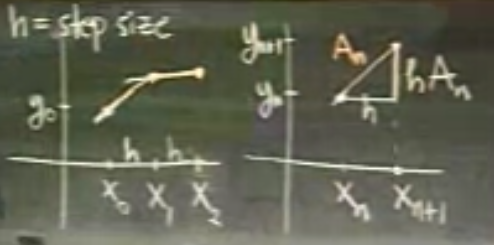
\includegraphics[height=4cm]{2_1.png}

Peki bahsedilen ODE baglaminda bir yere ``gitmek'' ne demektir? Takip ettigimiz,
cevap olarak odaklandigimiz $y$ fonksiyonudur. Unutmayalim ki bu fonksiyonun tam
hali $y(x)$, yani $y$, $x$'in bir fonksiyonu, $y$'nin turevi $y$'nin $x$'e gore
turevi demek. Turev egim demektir, egim fonksiyonun o noktadaki kabaca,
yaklasiksal bir yonudur. O yonu takip edersek o fonksiyonu asagi yukari takip
ediyoruz demektir.

Grafikte $h$ basamak mesafesi, yani $x$ uzerinde yaptigimiz sabit ziplama
mesafesi. Bu kordinatta hangi aralikla zipliyoruz? 0.1 mi, 1 mi, 5 mi? Bunun
secimini biz yapiyoruz. 

Euler Denklemleri bir adim icin soyle tanimlidir:

\[ x_{n+1} = x_n + h \]

\[ y_{n+1} = y_n + hA_n \]

\[ A_n = f(x_n, y_n) \]

Bu basamaklar ozyineli (recursive) olarak tanimlanir, bir sonraki adim, bir
onceki adimin degerlerini kullanir. 

Ornek

\[ y' = x^2 - y^2 \]

\[ y_1(0) = 1 \]

\[ h = 0.1 \]

Ustteki formul temel (elementary) fonksiyonlar kullanilarak cozulemez. O yuzden
Euler'in yontemi gibi bir numerik cozum burada uygun olur. 

\begin{tabular}{ccccc}
n & $x_n$ & $y_n$ & $A_n$ & $hA_n$ \\
\hline
0 & 0 & 1 & -1 & -0.1 \\
\hline
1 & .1 & .9 & -.80 & -0.08 \\
\hline
2 & .2 & .82 &  & 
\end{tabular}

$y$ icin eristigimiz sonuc .82 degeridir. Simdi sunu soralim: Bu cevap cok
yukarida mi cok asagida bir cevap mi? Pur numerik sonuclarda karsilasilan bir
problem budur, gercek cevabi analitik olarak bilmedigimiz icin ona ne kadar
yaklasip yaklasmadigimiz. Cevabi geometrik olarak verelim. Eger cozum bir duz
cizgi olsaydi, Euler metodu her bu cizgi uzerinde hep dogru cevabi veriyor
olurdu. 

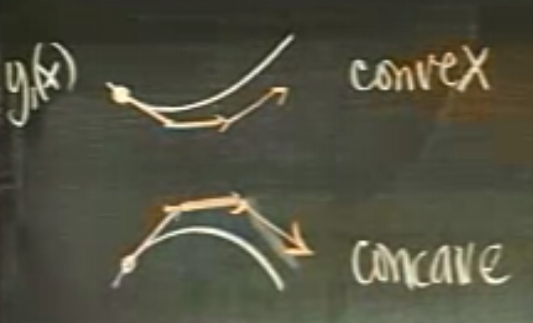
\includegraphics[height=4cm]{2_2.png}

Eger cozum disbukey (concave) olsaydi, ustteki gibi Euler metodu cok asagi
dusecekti. Ilk adimda fazla asagi inecekti, ve sonra bu hatadan donemeyecek, hep
esas fonksiyona uzak kalacakti. Icbukey olunca benzer sekilde, ama fazla
yukarida kalacakti. 

Peki elimizde bir analitik cevap olmadigina gore cevabin disbukey (convex) mi
icbukey mi (concave) olup olmadigini nereye bakarak anlayacagiz? Calculus tekrar
hizir gibi imdada yetisiyor. Ikinci turevi hatirlayalim: Eger $y'' > 0$ ise
birinci turev surekli artiyor demektir, yani $y$ disbukeydir. Eger $y'' < 0$ ise
tam tersi. Fakat hala bir problem var, analitik fonksiyon yok ise ikinci turevi
nasil hesaplayacagiz? Cevap: Diferansiyel fonksiyonun kendisini kullanarak.

$y' = x^2 - y^2$'nin turevini alirsak, 

$y'' = 2x - 2yy'$ sonucunu elde ederiz (turev alirken zincirleme kanununu
kullandigimiza dikkat).

O zaman baslangic noktasi $(0,1)$ de $y''$ nedir? $y'(0) = -1$, $y''= 2 \cdot 0
- 2\cdot 1 = 2$. 
Demek ki cozum baslangicta disbukey, ve Euler cozumunu uzun sureli takip
etmezsek cozumun cok altinda kalabiliriz. 

Tabii ki cozum bir dis bir ic olarak surekli degisen, dalgali bir yapida
olabilir, bu da mumkun. Burada asil gostermek istedigimiz diferansiyel denklemin
kendisini kullanarak cozum hakkinda analitik hicbir sey bilmeden onun hakkinda
nasil bilgi edinebilecegimizi gormektir. 

Hata Analizi

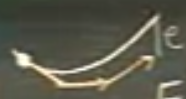
\includegraphics[height=2cm]{2_3.png}

Hata analizi Euler'in cozume ne kadar uzak kaldiginin hesabidir, yani $e$
sayisini hesaplamaktir. Bu degerin mutlak degeri (absolute value) kullanilir. 

Daha iyi sonuclar icin daha kucuk $h$ basamaklari kullanilabilir, o zaman sonuca
daha yakin kalabiliriz. O zaman $e$'nin $h$'ye bagli oldugunu
soyleyebiliriz. Formulsel olarak bu ifade suna benzer:

\[ |e \sim c_1 h| \]

Buna ifadeye gore Euler metotu birinci derece bir metottur denir, bu derecenin
ODE'nin derecesiyle alakasi yok, $h$'nin ustteki formulde hangi ustel formde
olduguyla alakali. Birincil derecede bir iliski mesela basamagi yarisina
indirince hatayi yarisina indirirmek demektir.

Euler metodundan daha bir yontem bulmak demek, egimi daha iyi hesaplayan bir
yontem bulmak demektir. Eger hatada rol oynayan en onemli faktor egim olduguna
gore, daha az hata icin daha iyi egim hesaplamak mantikli olacaktir. 

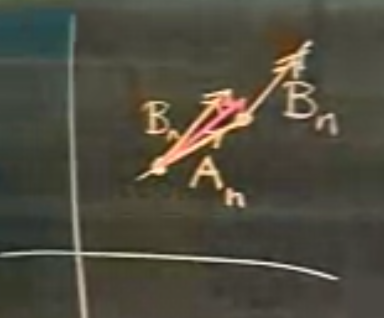
\includegraphics[height=4cm]{2_4.png}

Daha iyi egim nasil hesaplanir? Diyelim ki tek bir ziplama yerine iki kere
zipladik. Disbukey durumda birinci ziplamada cok asagi, ikincide biraz daha
yukari gidiyor olurduk, o zaman bunlarin ortalamasini alirsak, daha iyi bir egim
elde edebilirdik. 

\[ x_{n+1} = x_n + h \]

\[ \hat{y}_{n+1} = y_n + h A_n \]

\[ B_n = f(x_{n+1},\hat{y}_{n+1}) \]

\[ y_{n+1} = y_n + h(\frac{A_n+B_n}{2}) \]

Niye sapkali $y$ yani $\hat{y}$ kullandik? Cunku ortalama hesaplamak icin
aslinda n+1 noktasinda gecici bir deger hesapliyoruz, bu geciciligi gostermek
icin $\hat{y}$ ifadesini kullandik.

Bu metot Heun, Gelistirilmis Euler (Improved), Degistirilmis (Modified) Euler, RK2
gibi isimlerle anilir. RK2 Runga-Kutta'nin kisaltmasi, '2' ibaresi bu yontemin
ikinci dereceli bir metot olmasidir. Yani 

\[ e \sim c_2 h^2 \]

Basamagi yarisina indirmek hatayi dortte birine indirmek demektir. O zaman niye
bu metot her yerde kullanilmiyor? Cunku RK2 ile egim iki kere hesaplaniyor,
Euler ile bir kere, yani numerik kod iki kat daha fazla calismak, yani daha
yavaslamak zorundadir. 

RK4 da var, bu dorduncu seviyede bir metot. Egim soyle hesaplanir:

\[ \frac{A_n + 2B_n + 2C_n + D_n}{6} \]

Numerik Yontemlerde Bazi Tehlikeli Noktalar

1. Hoca odevde bizim kesfetmemizi istedi

2. Su basit denkleme bakalim: $y' = y^2$. Degiskenleri ayiralim ve analitik cevabi
$y=\frac{1}{c}$. O zaman bu denklemi numerik olarak cozerken alttaki grafik
takip ediliyor olacak.

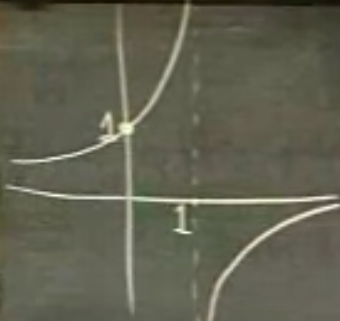
\includegraphics[height=4cm]{2_5.png}

Diyelim ki $y(0) = 1$'den basladik ve $y(2)$'i bulacagiz. Saga dogru yavas yavas
gidiyoruz ama problem, bu fonksiyon $y(1)$ degerinde sonsuza gidiyor. Demek ki
adim adim saga giden numerik cozum o noktayi hicbir zaman
asamayacaktir, sonsuzlukta kaybolacaktir. Bu tehlikeli noktayi onceden tahmin
edemez miydik? Hayir. Ustteki diferansiyel denklemin her cozumunun kendine has
bir tekilsel (singularity) noktasi vardir ve bundan sadece kendisi
haberdadir. 

\end{document}

